%%%%%%%% ICML 2018 EXAMPLE LATEX SUBMISSION FILE %%%%%%%%%%%%%%%%%

\documentclass{article}

% Recommended, but optional, packages for figures and better typesetting:
\usepackage{microtype}
\usepackage{graphicx}
\usepackage{subfigure}
\usepackage{booktabs} % for professional tables
\usepackage{amsmath}
\usepackage{amsfonts}
\usepackage{amssymb}
\usepackage{mathtools}
\usepackage{mathrsfs}
\usepackage{nicefrac}
\usepackage{amsthm}
\usepackage{thmtools}
\usepackage{thm-restate}
%\usepackage[ruled]{algorithm2e} % Comment out this line
\usepackage{array, makecell}
\usepackage{listings}
% hyperref makes hyperlinks in the resulting PDF.
% If your build breaks (sometimes temporarily if a hyperlink spans a page)
% please comment out the following usepackage line and replace
% \usepackage{icml2018} with \usepackage[nohyperref]{icml2018} above.
\usepackage{hyperref}
\newcommand\todo[1]{\textcolor{red}{#1}}

% Attempt to make hyperref and algorithmic work together better:
\newcommand{\theHalgorithm}{\arabic{algorithm}}

% Use the following line for the initial blind version submitted for review:
%\usepackage{icml2018_ift6269}

% If accepted, instead use the following line for the camera-ready submission:
\usepackage[accepted]{icml2018_ift6269}
% SLJ: -> use this for your IFT 6269 project report!

% The \icmltitle you define below is probably too long as a header.
% Therefore, a short form for the running title is supplied here:
\icmltitlerunning{Autoregressive VAE for Causal Modeling}

\begin{document}

\twocolumn[
\icmltitle{Autoregressive Variational Auto-Encoder for Causal Modeling}

% It is OKAY to include author information, even for blind
% submissions: the style file will automatically remove it for you
% unless you've provided the [accepted] option to the icml2018
% package.

% List of affiliations: The first argument should be a (short)
% identifier you will use later to specify author affiliations
% Academic affiliations should list Department, University, City, Region, Country
% Industry affiliations should list Company, City, Region, Country

% You can specify symbols, otherwise they are numbered in order.
% Ideally, you should not use this facility. Affiliations will be numbered
% in order of appearance and this is the preferred way.

\begin{icmlauthorlist}
\icmlauthor{Tom Marty}{udem,mi}
\end{icmlauthorlist}

\icmlaffiliation{udem}{Université de Montréal, Québec, Canada}
\icmlaffiliation{mi}{Mila, Quebec AI Institute}

\icmlcorrespondingauthor{Tom Marty}{tom.marty@mila.quebec}

% You may provide any keywords that you
% find helpful for describing your paper; these are used to populate
% the "keywords" metadata in the PDF but will not be shown in the document
\icmlkeywords{Machine Learning, ICML}

\vskip 0.3in
]

% this must go after the closing bracket ] following \twocolumn[ ...

% This command actually creates the footnote in the first column
% listing the affiliations and the copyright notice.
% The command takes one argument, which is text to display at the start of the footnote.
% The \icmlEqualContribution command is standard text for equal contribution.
% Remove it (just {}) if you do not need this facility.

\printAffiliationsAndNotice{} % otherwise use the standard text.

\begin{abstract}

Causal modeling is an active area of research that consist in inferring the functional components of a causal model from multi-intervention data. A causal model is made of independent mechanisms that govern the interactions between the different variables in the model. Recovering these causal mechanisms poses significant challenges because of the inherent confounding bias that can arise from the different interventional datasets considered. In this project, we propose to use a Variational auto-encoder with discrete latent in order to jointly estimate the interventional regimes and interventional targets of the data, required to deconfound the estimation of the independent causal mechanisms.

\end{abstract}
\section{Motivations}\label{subsec:intro}

\section{Background}\label{subsec:background}

In this section, we introduce some of the basic concepts that will be used in the rest of the report. We will first introduce the concept of Structural Causal Models (SCM), the concept of intervention on these structure, then quickly present the usual assumptions made in the causal modeling literature. If the reader is already familiar with these concepts, we recommend skipping directly to Section \ref{subsec:setting}.
\subsection{Structural Causal Models}

A Structural Causal Model (SCM) mathematically formalize the cause-effect relationships between the different random variables in a system. Precisely, an SCM is a triplet $\mathcal{S}(\mathcal{G},\mathbb{P}_{\boldsymbol{\epsilon}}, \mathcal{F})$ that defines the data-generating process of $N$ endogenous variables $\mathcal{X} = \left\{ X_1, X_2, \cdots, X_N \right\}$ and $N$ independent exogenous noise terms $\boldsymbol{\epsilon} = \left\{ \epsilon_1, \epsilon_2, \cdots, \epsilon_N \right\}$. It is composed of three terms :
\begin{itemize}
    \item A Directed Acyclic Graph \footnote{*commonly called a DAG} $\mathcal{G} = \left( \mathcal{V}, \mathcal{E} \right)$ that represents the causal structure of the model. Each node $X_i$ in the graph represent a random variable and each edge $X_i \rightarrow X_j$ represent a direct causal relationship between the two variables.
    \item A distribution over $N$ independent exogenous noise terms $\boldsymbol{\epsilon} = \left\{ \epsilon_1, \epsilon_2, \cdots, \epsilon_N \right\}$ that represent the unobserved factors influencing the endogenous variables.
    \item A set of $N$ mechanism $\mathcal{F} = \left\{ f_1, f_2, \cdots, f_N \right\}$ that represent the functional form of the causal relationships between the variables in the model. Each variable $X_i$ is a function of its parents $\text{Pa}(X_i)$ defined by the DAG and some exogenous noise $\epsilon_i$ sampled from $\mathbb{P}_{\boldsymbol{\epsilon_i}}$ :
    \begin{equation}
    X_i  = f_i(\text{Pa}(X_i), \epsilon_i)  \quad \epsilon_i \sim \mathbb{P}_{\epsilon_i}
    \end{equation}
\end{itemize}

This formulation induces a set of conditional probability distributions $p(X_i | \text{Pa}(X_i))$ such that the joint distribution over the variables $X$ can be expressed as a product of these conditional distributions:
$$p(X) = \prod_{i = 1}^N p(X_i | \text{Pa}(X_i)).$$
For the rest of this report, we will consider the variables $X_i$ and $\epsilon_i$ to be univariate.

\subsection{interventions and targets}
An important concept in the field of Causality is the notion of \textbf{intervention}. An intervention $\mathcal{I}$ is a modification of the data-generating process of a causal model $\mathcal{S}$ that consist in modifying a set of mechanisms $f_i \in \mathcal{F}_{\mathcal{I}}$ :

\begin{equation}
    f_i(\text{Pa}(X_i), \epsilon_i) \rightarrow f_i^{\mathcal{I}}(\text{Pa}(X_i), \epsilon_i) \quad \forall i \in \mathcal{F}_{\mathcal{I}}
\end{equation}
For a given intervention, the \textbf{targets} refers to the set of variables in the causal model whose mechanisms are altered by the intervention. There are different types of interventions that can be considered, we usually consider \textit{single} intervention where the set $\mathcal{F}_{\mathcal{I}}$ is reduced to a single altered mechanism, we refer the reader to \citet{Pearl_2009} for a more detailed discussion on interventions.

\paragraph{interventional regime}
Another important notion is the notion of interventional regime, which caracterise a set of samples $D_{\mathcal{I}_k}$  that were generated under the same intervention $\mathcal{I}_k$. Additionally, when no intervention is applied, the data is said to be generated under the observational regime $D_{\mathcal{O}}$.

\paragraph{interventional Faithfulness} First introduced by \citet{chevalley2024derivingcausalordersinglevariable}, this assumption guarantees that any valid intervention $\mathcal{I}_k$ should significantly alter the distribution of the downstream nodes of the intervened mechanism such that inversely inferring the possible intervention from the downstream nodes is possible.

\section{Setting}\label{subsec:setting}

In causal modeling, given a dataset $\mathcal{D}$ generated from an SCM $\mathcal{S}= (\mathcal{G}, \mathbb{P}_{\boldsymbol{\epsilon}}, \mathcal{F})$, the goal is usually to retrieve full knowledge about $\mathcal{S}$. In \textit{Causal Discovery}, the challenge is to infer the graph $\mathcal{G}$, which is a particularily harduous task because of the inherent difficulties arising from discrete optimization (a graph a is discrete structure) under constraint (e.g. Acyclicity). In \textit{Causal Modelling}, the goal is to learn the mechanisms $\mathcal{F}$. Depending on what is to be learned, different assumptions have to be made on the data-generation process in order to identify the causal model. These assumptions can be summarized as follows:
\begin{enumerate}
    \item unknown/known interventional regime
    \item unknown/known single/multiple interventional targets
    \item unknown/known graph structure
    \item restricting assumptions on the mechanisms (e.g. Additive noise, linear mechanisms, gaussian noise...)
\end{enumerate}

In this project, we will consider a slightly unusual setting :

We consider a dataset $\mathcal{D} = \left\{ D_{\mathcal{O}},D_{I_1}, \cdots, D_{I_N} \right\}$ composed of samples generated under $N$ different interventional regimes. Each regime is obtained by performing a soft intervention on a single mechanism. Each mechanism is intervened only once, meaning that there are $N$ mechanisms and $N$ corresponding interventions. Finally, we consider \textbf{that the graph $\mathcal{G}$ is known}. We discuss the relevance of such a specific setting in Section \ref{subsec:Relevance}.
 The subtlety of our setting is that the data is completely shuffled such that for each sample $X \in \mathcal{D}$ neither the interventional regime it belongs to nor the interventional target of this regime is known. Finally, the task consist in modeling each of the mechanisms $f(X_i | \text{Pa}(X_i))$ under both the observational regime and each of the interventional regimes.

We treat this problem as a latent-variable model where the latent variables are the interventional regime and the interventional target of each sample. Given that we usually don't know the functionnal form of the mechanisms of the causal model, the posterior distribution over the latent variables is most of the time intractable. For this reason, we will use a Variational Auto-encoder (VAE) to approximate the posterior distribution over the latent variables. We refer the reader to Section \ref{subsec:Method} for a more detailed explanation of the method.

\subsection{Relevance}
Why is it interesting ? show that with counter example saying retrieving the observational regime exactly is tricky.

Known graph is a pretty strong assumption, but we argue that this problem remains not trivial.

In this setting, it is not trivial to infer each mechanism under observational regime $p_{obs}(X_i | \text{Pa}(X_i))$ of the causal model $\mathcal{M}$, because the straightforward maximisation of data-loglikelihood will yield probabilistic models $\hat{p_{obs}}(X_i | \text{Pa}(X_i))$ that will be biaised by samples for which the true mechanism $p_{obs}(X_i | \text{Pa}(X_i))$ was in fact not in its observational form : $p_{obs} \rightarrow p_{int}$. In order to unbiaise this estimate, we therefore need to account for these possible interventions by also modeling and estimating the state of each mechanism using a boolean variable $z_i$. Recalling that some samples share some dependencies since they were sampled under the same interventional regime, we can also infer the regime trough a variable $I_k$ and  leverage that shared characteristic to better encode the interventions.

We could represents this data-generation process with a latent-variable model where the unknown latent are boolean variables representing the state of each mechanisms (\textit{unintervened} / \textit{intervened}). In this setting, we are trying to jointly infer the latent variables and the parameters $\theta$ of our statistical model $\hat{p_{obs}}$. To this end, we will use the variational-EM algorithm.

\begin{figure}
\centering
    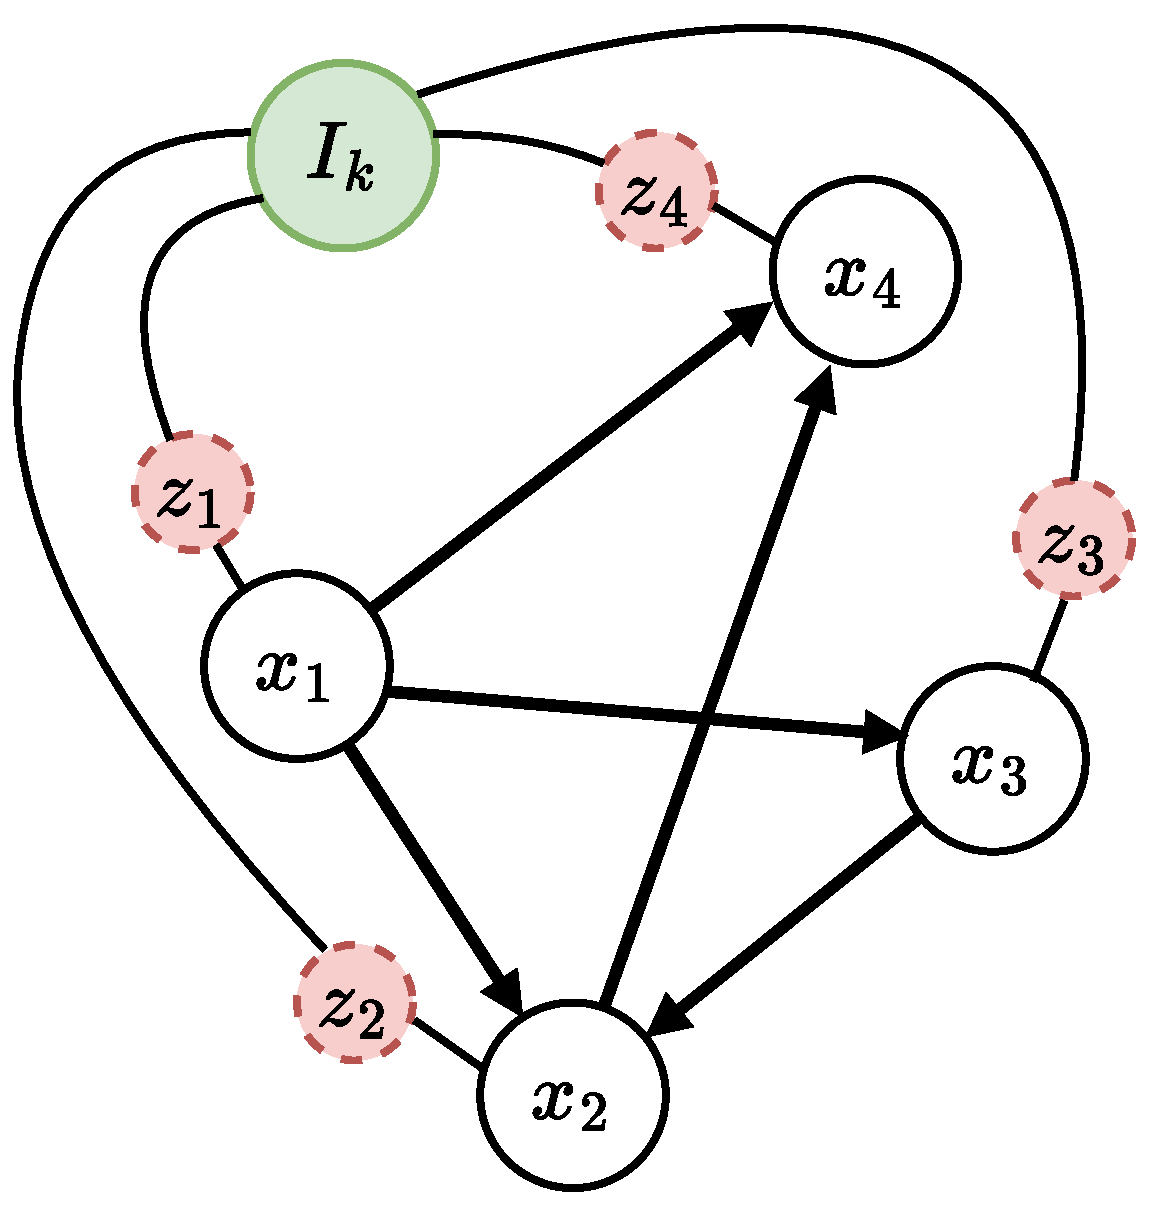
\includegraphics[width=0.2\textwidth]{images/DAG.pdf}
    \caption{Graphical model of the data-generation process augmented with the unobserved latent variables. $I_k$ represent the interventional regime and the $z_i \; i \in [1,N]$ are boolean variable that encode the state of each mechanism $p(X_i | \text{Pa}(X_i))$}.
    \label{fig:DAG}
\end{figure}

\paragraph{Outline} First, we will be discussing the validity of the assumptions made in the data-generation process alongside the ones made on the probabilistic model, then we will derive the EM algorithm itself and explain the necessity for the variational variant of EM. Finally we will run our method on a set of controlled experiments, and discuss the results when compared with other methods for causal modeling.


\section{Method}\label{subsec:Method}

In this problem we are trying to learn a generative model of the data under unobserved interventions, for this purpose we will use a Variational Auto-encoder \citep{kingma2022autoencodingvariationalbayes}
with discrete latent variables, the decoding will take profit of the known graph structure to reconstruct the variables $X_i$ from their sampled parents $\text{Pa}(X_i)$, in an autoregressive fashion.
. In this setting the latent variables are the interventional target $z_i \quad i \in [1,N]$ of each sample $x$. In order to faithfully model the data-generation process,
A VAE is a general framework for solving statistical modeling problem with unobserved latent variables. Given a data point $x$, the Variational Auto-encoder (VAE) is tasked to learn an approximate posterior distribution over these latent variables $q_\phi(z | x)$. Basically, the algorithm consist in maximizing the \textbf{evidence lower bound (ELBO)}, a lower bound of the log-likelihood of the data defined as follows :
\begin{align*}
    &\quad\quad \log p_\theta(x) \geq  \\
    & \underbrace{ - \text{KL}\left(q_\phi(z | x) \,||\, p_\theta(z)\right)+ \mathbb{E}_{q_\phi(z | x)} \left[ \log p_\theta(x | z) \right]}_{\text{ELBO}}
\end{align*}

In this optimization problem, we want to find the parameters $\theta$ and $\phi$ that maximize the ELBO. $q_\phi(z | x)$ is the approximate posterior distribution over the latent variables and $\phi$ defines the variational family of distributions used to approximate the posterior. $p_\theta(z)$ is the prior distribution over the latent variables and $p_\theta(x | z)$ is the likelihood of the data given the latent variables. We refer to figure \ref{fig:architecture} for a representation of the full architecture of the model.
\begin{figure}
\centering
    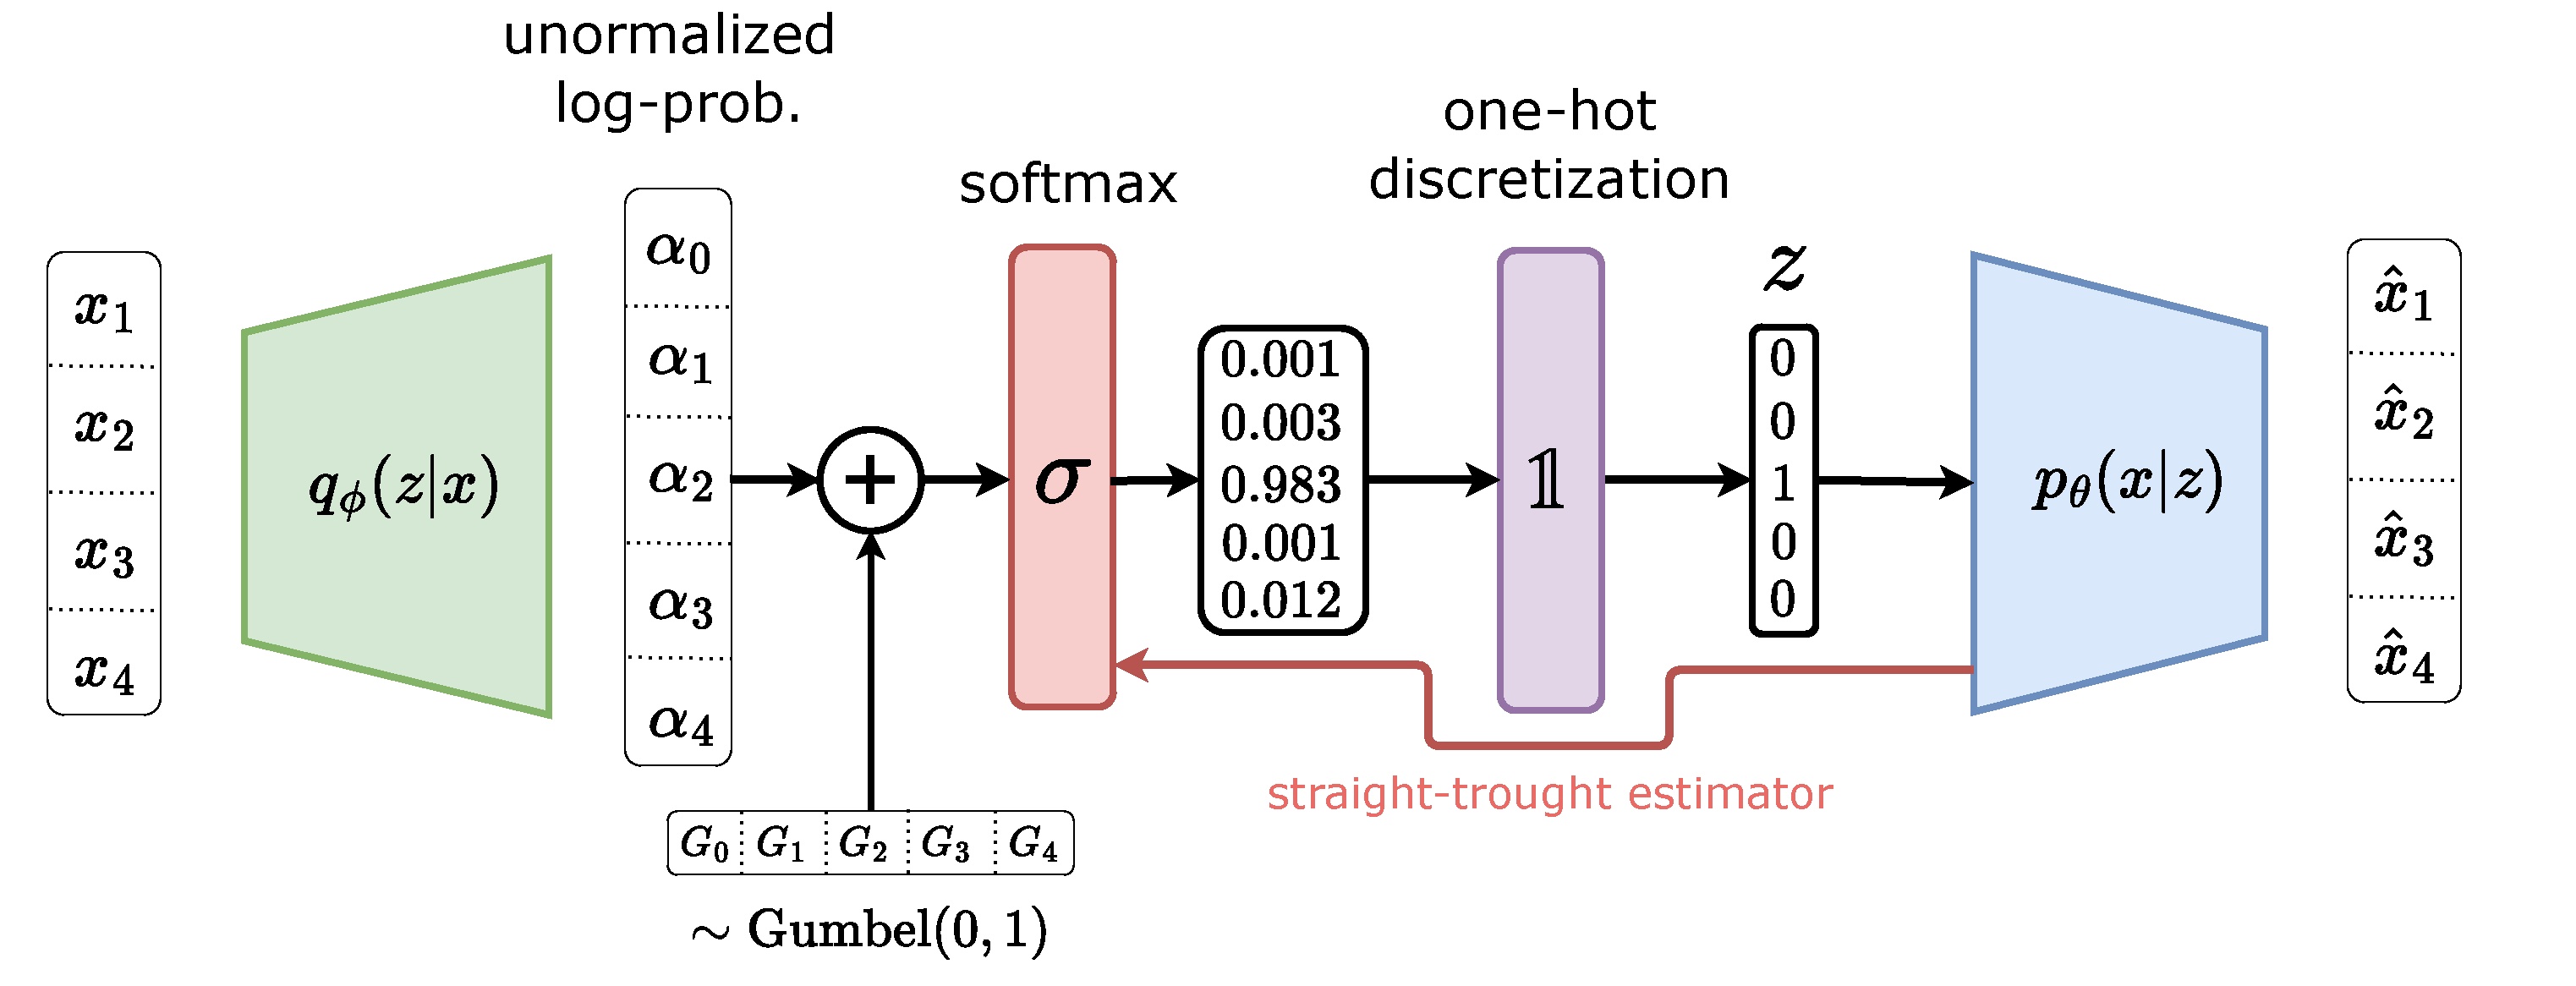
\includegraphics[width=0.48\textwidth]{images/architecture.pdf}
    \caption{Architecture of the Variational Auto-Encoder. An encoder takes as input the data $x$ and outputs the parameters of the approximate posterior categorical distribution $q_\phi(z | x)$. The sampled discrete latent variables $z$ are then fed to the decoder that outputs the parameters of the likelihood distribution $p_\theta(x | z)$. During backpropagation, the discrete latents are approximated using the Gumbel-Softmax reparametrization trick. For more details on the architecture of the likelyhood model $p_\theta(x | z)$, we refer to Figure \ref{fig:architecture_decoder}.}
    \label{fig:architecture}
\end{figure}
\paragraph{Regime Learning ($q_\phi(z | x)$)}Given that for each mechanism $f_i$, we have a set of samples $D_{\mathcal{I}_k}$ that were generated under the same intervention $\mathcal{I}_k$, we can leverage this shared characteristic to better encode the interventions. We therefore propose to use a boolean latent variable $z_i$ that encodes the state of each mechanism $f_i$ (intervened or not intervened). We use the following formulation : $\tilde{z} \sim \mathcal{B}(\pi_\phi(x))$ and $z = \text{one-hot}(\tilde{z})$, where $\mathcal{B}$ is a multinoulli distribution parameterized by $\pi_\phi(x)$, the output of a neural network that predict the probability of each mechanism to be intervened.



\paragraph{Prior distribution ($p_\theta(z)$)} We will use a uniform prior over the latent variables $z$. \todo{justify}. We can now derive the Kullback-Leibler divergence term of the ELBO :
\begin{align*}
    -\text{KL}\left(q_\phi(z | x) \,||\, p_\theta(z)\right)
    &= - \sum_{i} \pi_\phi(x)_i \log \frac{\pi_\phi(x)_i}{p_\theta(z_i)} \\
    &= - \sum_{i} \pi_\phi(x)_i \log \frac{\pi_\phi(x)_i}{1/N} \\
    &= - \sum_{i} \pi_\phi(x)_i \log \pi_\phi(x)_i - \log N \\
    &= \text{H}(\pi_\phi(x)) - \log N
\end{align*}
\paragraph{Mechanism Learning ($p_\theta(x | z)$)}

Given that the graph $\mathcal{G}$ is known, we can use the following factorization of the likelihood :
\begin{align*}
    p_\theta(x | z) &= \prod_{i = 1}^N p_\theta(x_i | \text{Pa}(X_i), z_i) \\
    &= \prod_{i = 1}^N p_\theta(x_i | \text{Pa}(X_i), z_i)
\end{align*}

We will use a neural network to model the conditional distribution $p_\theta(x_i | \text{Pa}(X_i), z_i)$ for each mechanism $f_i$. Specifically, $p_\theta(x_i | \text{Pa}(X_i), z_i) = \mathcal{N}(\mu_\theta(x_i, \text{Pa}(X_i), z_i), 1)$ where $\mu_\theta(x_i, \text{Pa}(X_i), z_i)$ is the output of a neural network that takes as input the parents of $X_i$ and the infered state of the mechanism $z_i$. We chose to model the likelihood as a gaussian distribution with unit variance because it allows to account for the stochasticity of the exogenous variable $N_i$ while keeping the optimization of the ELBO simple. Specifically, the likelihood term of the ELBO can be written as follows :
\begin{align*}
    & \quad \mathbb{E}_{q_\phi(z | x)} \left[ \log p_\theta(x | z) \right] \\ &\simeq \underbrace{\frac{1}{L} \sum_{l = 1}^L }_{\text{n latent samples}} \sum_{i = 1}^N \log \mathcal{N}(x_i | \mu_\theta(x_i, \text{Pa}(X_i), z_i), 1)\\
    &\simeq \frac{1}{L} \sum_{l = 1}^L \sum_{i = 1}^N \left( -\frac{1}{2} \left( x_i - \mu_\theta(x_i, \text{Pa}(X_i), z_i) \right)^2 \right) + \text{const.}
\end{align*}
Maximizing the expected log-likelihood of the data under the model is equivalent to minimizing the MSE loss for each mechanism of the causal model. In practice, when considering large enought mini-batch, we can use single-sample Monte-Carlo estimation $L=1$ to limit the computational cost of the ELBO optimization.

\todo{talk about Autoregressive stuff}
\begin{figure}
\centering
    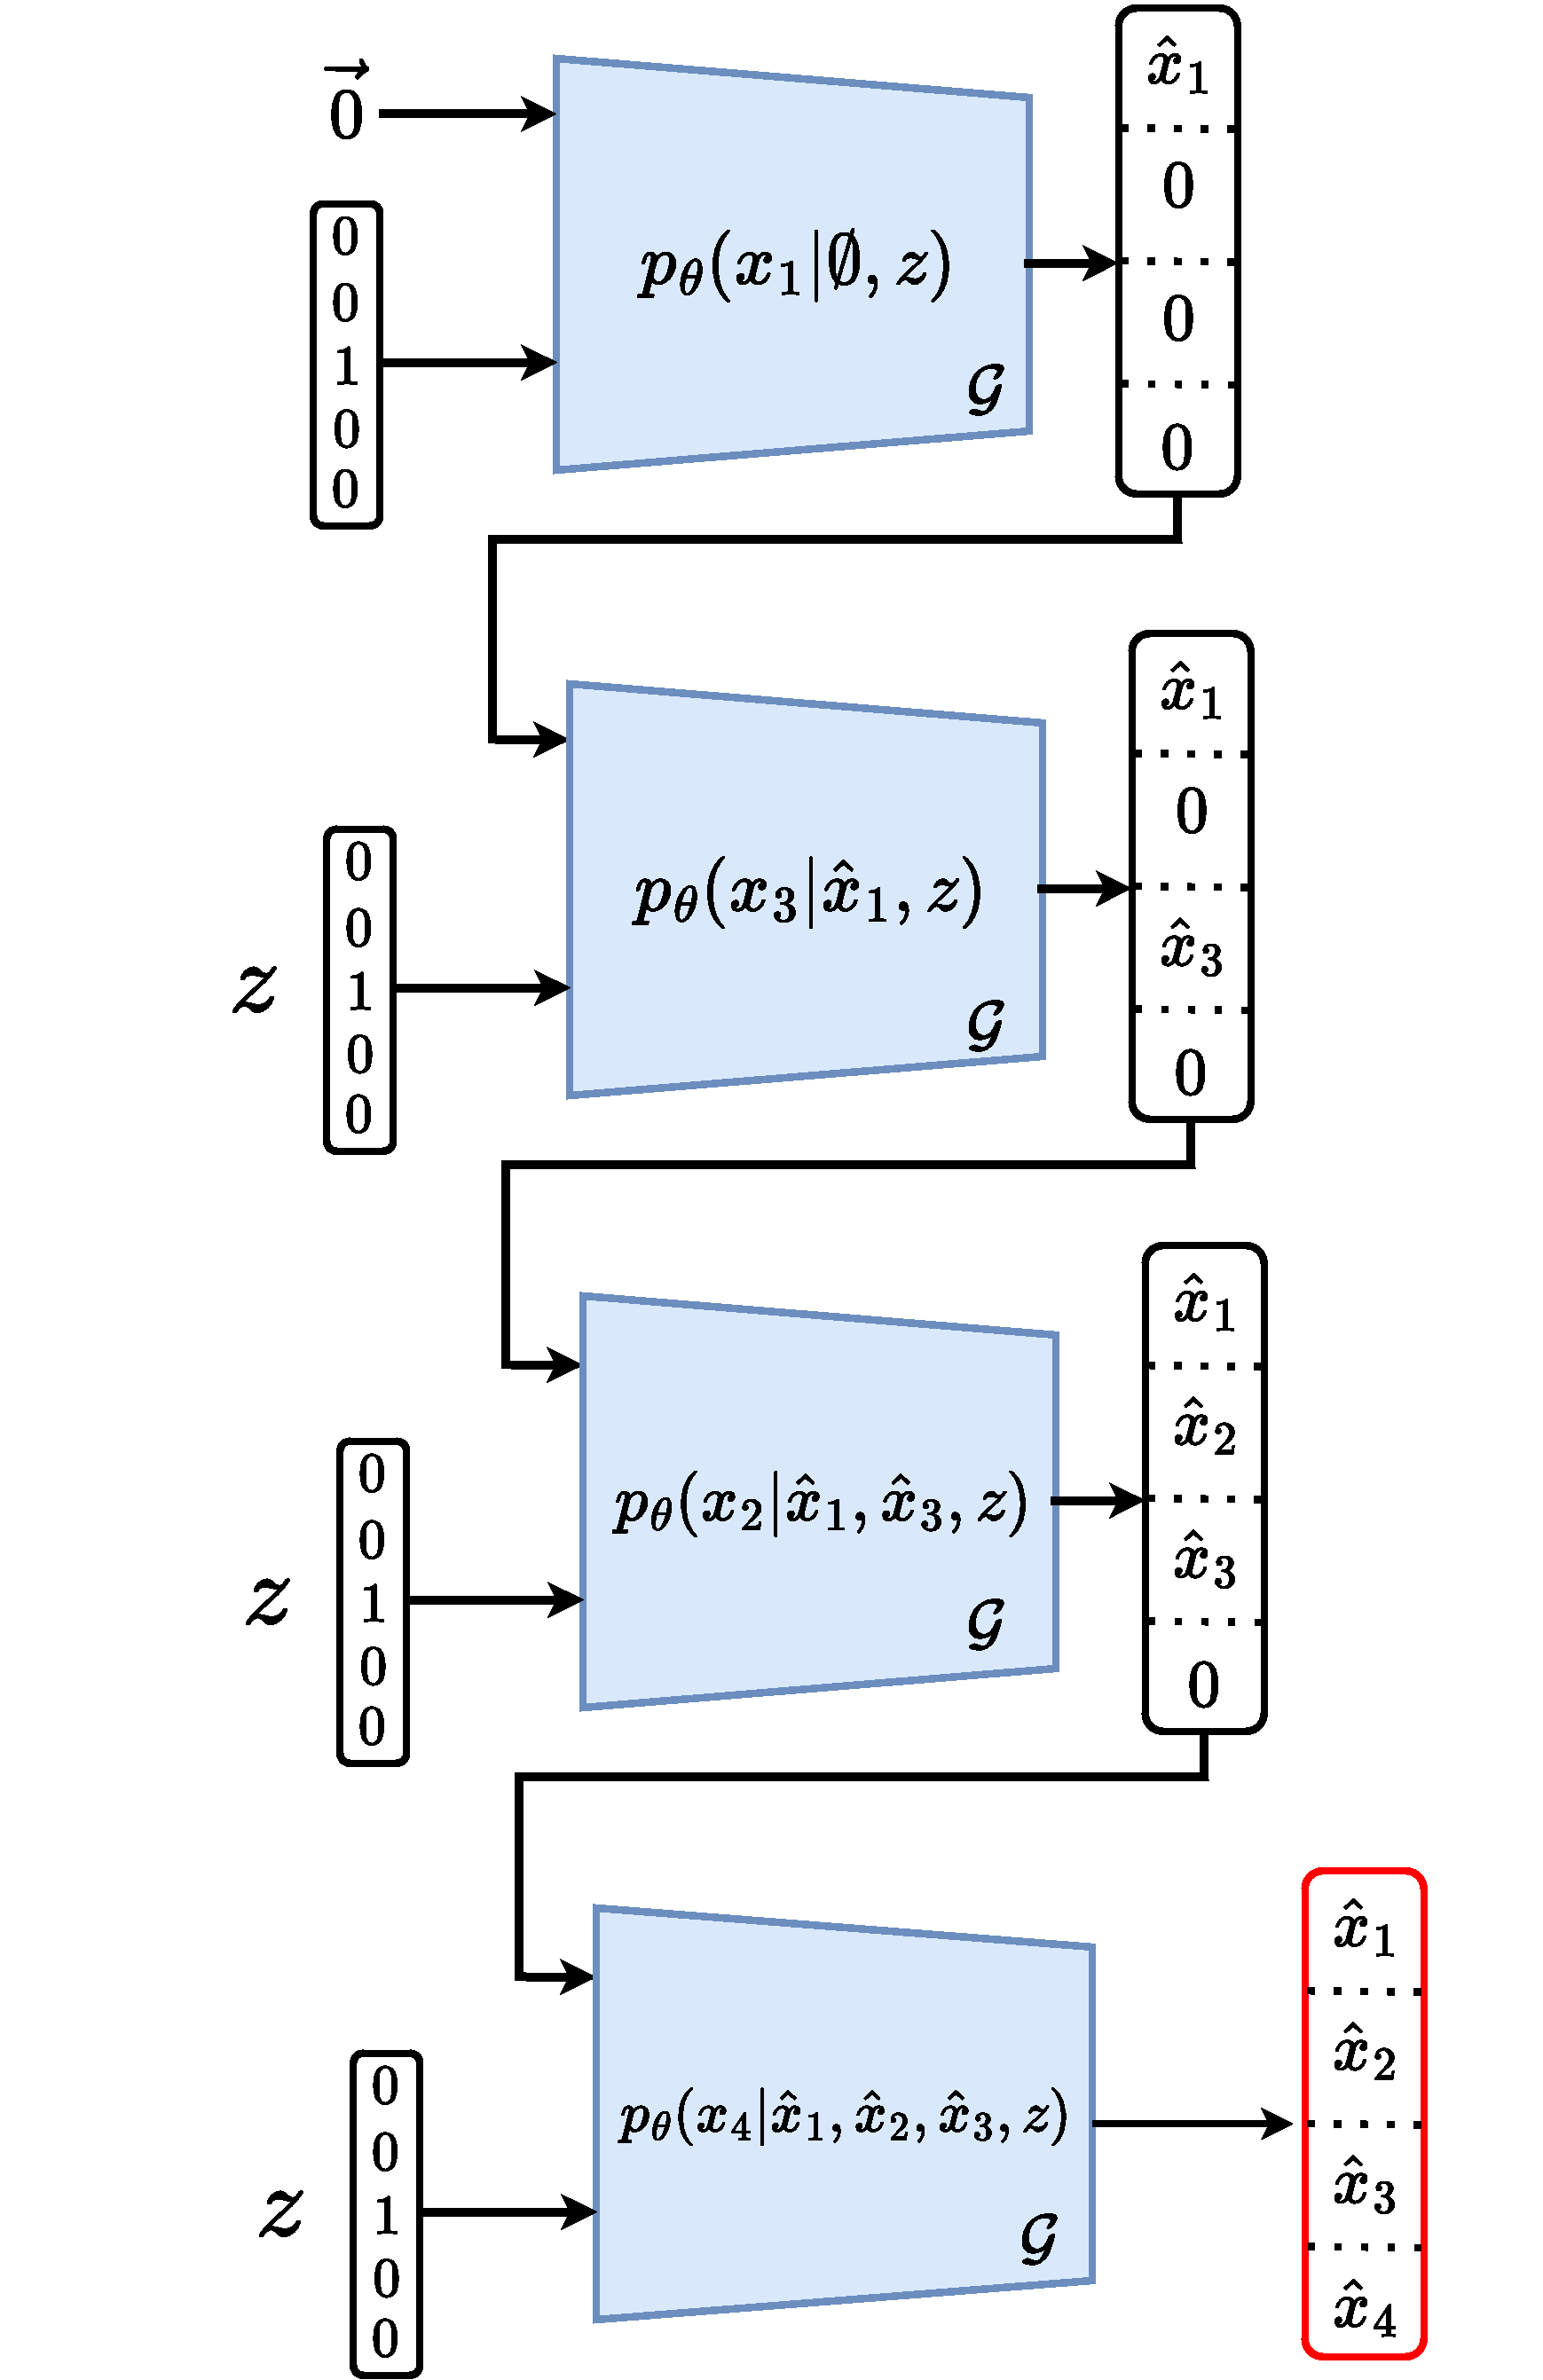
\includegraphics[width=0.35\textwidth]{images/architecture_decoder.pdf}
    \caption{Architecture of the likelihood model $p_\theta(x | z)$. Each mechanism $f_i$ is modeled as a gaussian distribution with mean $\mu_\theta(x_i, \text{Pa}(X_i), z_i)$ and unit variance. The mean of the input sample is reconstructed autoregressively following the topological order of the graph $\mathcal{G}$.}
    \label{fig:architecture_decoder}
\end{figure}
\paragraph{discrete reparametrization trick}
The latent variable $z$ lies in a discrete space, which makes the objective non-differentiable with respect to the sampling process $q_\phi(z | x)$. For this reason, we will use the Gumbel Softmax reparameterization trick \citep{jang2017categoricalreparameterizationgumbelsoftmax} to make the sampling process differentiable while keeping the discrete nature of the latent variables.
 \todo{add a section in poster  : why I made these choice}
\section{Experiments}\label{subsec:Experiments}
In this section, we discuss the experiments that we run to evaluate the performance of our model at infering the right regimes and learning the mechanisms of the causal model. We will first describe the data-generation process, then we will present the evaluation metrics used to assess the performance of our model. We will Additionally run an ablation study to evaluate the necessity of some of the assumption we made in the data-generation process

Compared to the standard EM for which a closed form update does not always exist, Variational methods allows to describe a wider variety of posterior distributions, allowing to tackle more complex (i.e. realistic) problems.\footnote{ANM are not realistic, but they are a good starting point to evaluate the performance of our model.}


\subsection{Data-generation process}

To evaluate our model, we need a dataset that was generated from a known causal model. In this project, we consider that the SCM that generated the data is additive noise model (ANM) with linear mechanisms. The data is generated as follows : We have $N$ variables $X = \left\{ X_1, X_2, \cdots, X_N \right\}$.  The DAG $\mathcal{G}$ is sampled from a Erdos-Renyi DAG distribution with a fixed probability of edge $p$. Given that structure, the mechanisms $f_i$ are defined as linear functions of their parents and the exogenous noise terms :
\begin{equation}
    X_i = \sum_{j \in \text{Pa}(X_i)} w_{ij} X_j + \epsilon_i
\end{equation}
In order to satisfy the faithfulness assumption, we sample the weights $w_{ij}$ from a truncated uniform distribution $w_{ij} \sim \mathcal{U}(-1,0.1) \cup \mathcal{U}(0.1,1)$. In practice, even if this assumption is not verified, the model should still be able to ignore the unfaitful parents and learn the right mechanisms. The exogenous noise terms $\boldsymbol{\epsilon}$ are sampled from a standard normal distribution.

\subsection{Evaluation metrics}
\todo{when the internvention are not strong enough, the latent features collapses during training, this is because even tought z was informative, there not much gain in predictive power since the two distribution are almost the same.}

\todo{Am I giving the right information the my decoder ?}

\todo{VAE is learning smtg (latent don't collapse) but the model is not able to identify the right regime for each sample and the reconstruction loss don't go to zero, while it should in theory.}

\section{Conclusion}\label{subsec:Conclusion}

In this project, we propose to tackle the problem of causal modelling under unknown interventions and regime as a latent variable model. We use a Variational Auto-encoder with discrete latent variables to jointly infer the interventional regime. It is too early to draw strong conclusion on the ability of our method to systematically identify the regime, but we can already see that some assumptions on the DGP are necessary to avoid latent variable collapse.

\bibliography{references}
\bibliographystyle{icml2018}

\end{document}


% This document was modified from the file originally made available by
% Pat Langley and Andrea Danyluk for ICML-2K. This version was created
% by Iain Murray in 2018. It was modified from a version from Dan Roy in
% 2017, which was based on a version from Lise Getoor and Tobias
% Scheffer, which was slightly modified from the 2010 version by
% Thorsten Joachims & Johannes Fuernkranz, slightly modified from the
% 2009 version by Kiri Wagstaff and Sam Roweis's 2008 version, which is
% slightly modified from Prasad Tadepalli's 2007 version which is a
% lightly changed version of the previous year's version by Andrew
% Moore, which was in turn edited from those of Kristian Kersting and
% Codrina Lauth. Alex Smola contributed to the algorithmic style files.
